% !TeX root = ../final.tex
% Revised one-hour lecture script.
% Teaching arc: INTERROGATE A MODEL.

\chapter{Learning chemistry from models}

\begin{notebox}
  \keypoint{What do you need to learn from this chapter?}
  A model can predict, classify, rank, or expose a pattern without explaining why the chemistry behaves in that way.
  By the end of this chapter, you should be able to distinguish interpolation from several forms of extrapolation, choose validation that matches a chemical claim, use residuals and reactivity cliffs to generate experiments, and explain why independent chemical evidence is required before a statistical relationship becomes a mechanistic argument.
\end{notebox}

% Suggested timing: 0--6 min
\section{The computer says this. Should we believe it?}

Chapter~5 ended with a fitted relationship between molecular representation and chemical response.
We now imagine that the model has returned a prediction for a new reaction.
The numerical value arrives with several questions hidden inside it:

\begin{itemize}
  \item Does the proposed reaction resemble the training chemistry in the representation used by the model?
  \item Was that kind of novelty tested during validation?
  \item Is the predicted response inside or outside the observed response range?
  \item Could the catalyst, substrate, phase, or mechanism change regime?
  \item Is the model being used to predict an outcome or to explain its cause?
\end{itemize}

\solution{4.5cm}{%
  \textbf{Initial judgement.} A model reports $92\%$ ee for a new catalyst. Write three reasons why the number might be unreliable even if the reported random-test error is small.
  \begin{itemize}
    \item the catalyst may be outside the represented training space;
    \item a random split may have tested only familiar catalyst and substrate families;
    \item the new catalyst may change speciation or mechanism;
    \item the representation may omit a relevant conformational or substrate-specific effect;
    \item analytical or data-selection bias may make the original error estimate optimistic.
  \end{itemize}
}

The purpose of interrogation is not to reject modelling.
It is to turn a model output into a chemical question that can be tested.

% Suggested timing: 6--16 min
\section{What kind of novelty is this?}

The word ``extrapolation'' is often used as though it described one operation.
In chemical modelling, several distinct forms of novelty can occur.

\subsection{Interpolation in a chosen representation}

A candidate is interpolative when it lies between well-supported training regions in the representation relevant to the model.
This is not an intrinsic label carried by the molecule.
Change the descriptors and the apparent neighbourhood can change.
A catalyst that is close in a fingerprint space may be distant in a conformer-aware steric space.

\subsection{Response-range extrapolation}

A prediction can lie beyond the highest or lowest response value observed during training.
For example, a catalyst inside the represented catalyst space may be predicted to give a selectivity higher than any training reaction.
Zahrt and co-workers deliberately tested this kind of prediction.
Its risk is different from asking the model to evaluate a new catalyst scaffold.

\subsection{Component and scaffold extrapolation}

A reaction assembled from familiar components can still be an unseen row.
A genuinely new substrate family, catalyst scaffold, reagent class, or solvent family asks a stronger question.
Component-held-out and scaffold-held-out tests estimate performance for that form of novelty more directly than random reaction splits.

\subsection{Mechanistic extrapolation}

The most dangerous case can look numerically ordinary.
A point may sit near training examples in descriptor space while crossing a boundary in ligation state, aggregation, rate-determining step, phase behaviour, or decomposition pathway.
The model then treats two chemical regimes as one smooth relationship.

\solution{5.2cm}{%
  \textbf{Place each case on a novelty map.} Draw two axes labelled ``distance in the chosen representation'' and ``change in chemical regime''.\\[0.5em]
  Add:
  \begin{enumerate}
    \item a new combination of familiar catalyst and substrate;
    \item a new catalyst scaffold with a familiar predicted selectivity;
    \item a familiar ligand that changes metal ligation state;
    \item a catalyst inside the training space predicted beyond the observed selectivity range.
  \end{enumerate}
  Which risk is visible to an ordinary distance calculation, and which requires chemical evidence?
}

\begin{conceptbox}
  \keypoint{Applicability domain is a chemical claim supported by numerical evidence.}
  It depends on the sampled chemistry, the representation, the response, the model, and the kind of novelty actually tested.
\end{conceptbox}

% Suggested timing: 16--24 min
\section{Read the errors chemically}

A residual is the difference between an observed response and its prediction,

\begin{equation}
  e_i=y_i-\hat{y}_i.
\end{equation}

A single summary metric discards the identities of the reactions that generated those residuals.
For chemical interpretation, those identities matter.

Small residuals scattered without obvious pattern are consistent with the model capturing the dominant relationship in the sampled domain.
A group of positive residuals for one substrate family means that the model systematically underpredicts that family.
Residuals that increase at one temperature range may indicate missing curvature, a measurement issue, or a change in regime.
One isolated large residual may be an experimental error, an unusual molecule, or the most chemically informative point in the dataset.

\solution{5.0cm}{%
  \textbf{Annotate a residual plot.}
  \begin{itemize}
    \item mark a random cloud around zero;
    \item draw a curved pattern that suggests a missing nonlinear term;
    \item colour one substrate family with consistently positive residuals;
    \item circle one extreme point and list the checks needed before deleting it.
  \end{itemize}
}

The correct response to an outlier is not automatically removal.
First verify sample identity, reaction execution, calibration, peak assignment, data processing, and whether the point belongs to the intended domain.
If the measurement is valid, the residual may reveal missing chemistry.

Reactivity cliffs are an extreme version of this idea.
A smooth model assumes that nearby inputs tend to have nearby outputs.
A cliff occurs when a small change in representation accompanies a large change in outcome.
That may indicate that the representation is poor, that a categorical distinction has been compressed into a continuous descriptor, or that the chemistry has crossed a mechanistic boundary.

% Suggested timing: 24--39 min
\section{Case study: a reactivity cliff becomes a chemical hypothesis}

Newman-Stonebraker and co-workers analysed 11 nickel- and palladium-catalysed cross-coupling datasets using descriptors for monodentate phosphine ligands.\mcite{NewmanStonebraker2021}
The objective was not simply to obtain the lowest prediction error.
It was to ask whether a general structural feature separated reactive and unreactive ligand regimes.

\subsection{Start with the experimental pattern}

Across the datasets, some ligands supported productive cross-coupling while apparently similar ligands did not.
A conventional cone angle did not give one useful boundary across the systems.
The descriptor that did was the minimum percent buried volume, $\%V_{\mathrm{bur}}(\min)$, evaluated across the accessible conformer ensemble.
A threshold close to $32\%$ separated active and inactive regions in multiple datasets.

\begin{figure}[htbp]
  \centering
  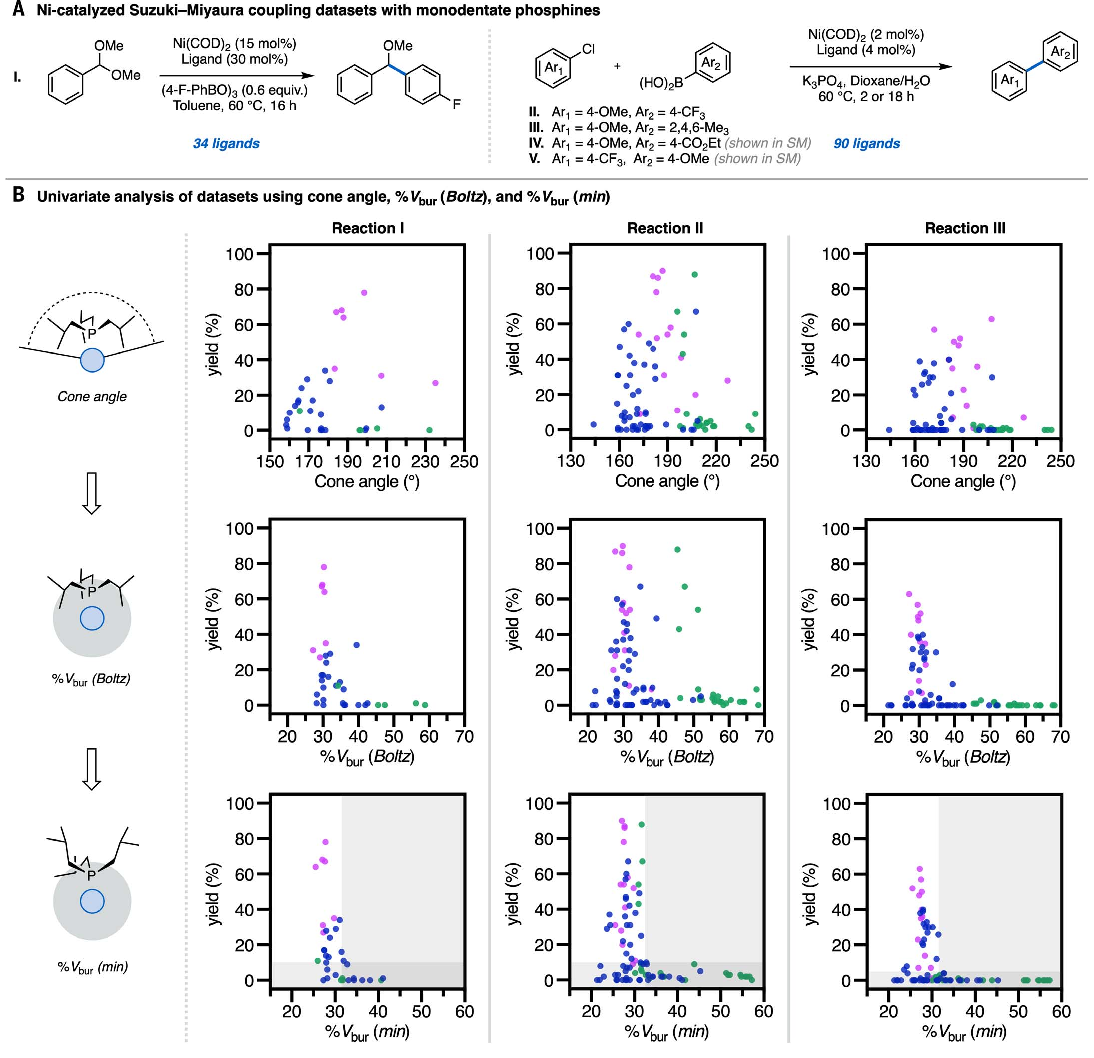
\includegraphics[width=\textwidth,height=0.70\textheight,keepaspectratio]{figures/chapter06-interrogate/01-newman-stonebraker-reactivity-cliffs-fig2.pdf}
  \caption{Phosphine reactivity datasets plotted against steric descriptors. The minimum buried volume reveals a recurring activity boundary that is obscured by other steric summaries. Reproduced from Newman--Stonebraker \textit{et al.}, \textit{Science} (2021), Fig.~2.}
  \label{fig6-newman-cliff}
\end{figure}

\solution{4.2cm}{%
  \textbf{Annotate the reactivity-cliff figure.}
  \begin{itemize}
    \item draw the approximate $\%V_{\mathrm{bur}}(\min)$ threshold;
    \item label the active and inactive regimes;
    \item identify ligands close to the boundary;
    \item mark any point that the one-variable rule misclassifies.
  \end{itemize}
}

At this stage, the model has produced a reproducible classification rule.
It has not yet explained why the rule works.
A numerical boundary might correlate with ligand family, donor ability, synthetic history, or another unmeasured property.

\solution{3.5cm}{%
  \textbf{Does the threshold establish mechanism?}\\[0.5em]
  No. It generates a hypothesis: the steric boundary may control the number of phosphines accommodated at the metal, changing catalyst ligation state and reactivity.
  Write down an experiment that probes ligation state independently of the reaction-yield model.
}

\subsection{Test the chemical hypothesis independently}

The authors used organometallic and spectroscopic studies to connect the descriptor boundary to phosphine ligation state.
The minimum-buried-volume threshold distinguished conditions under which bisligated and monoligated metal species were favoured.
That evidence gives the statistical cliff a chemical interpretation.

\begin{figure}[htbp]
  \centering
  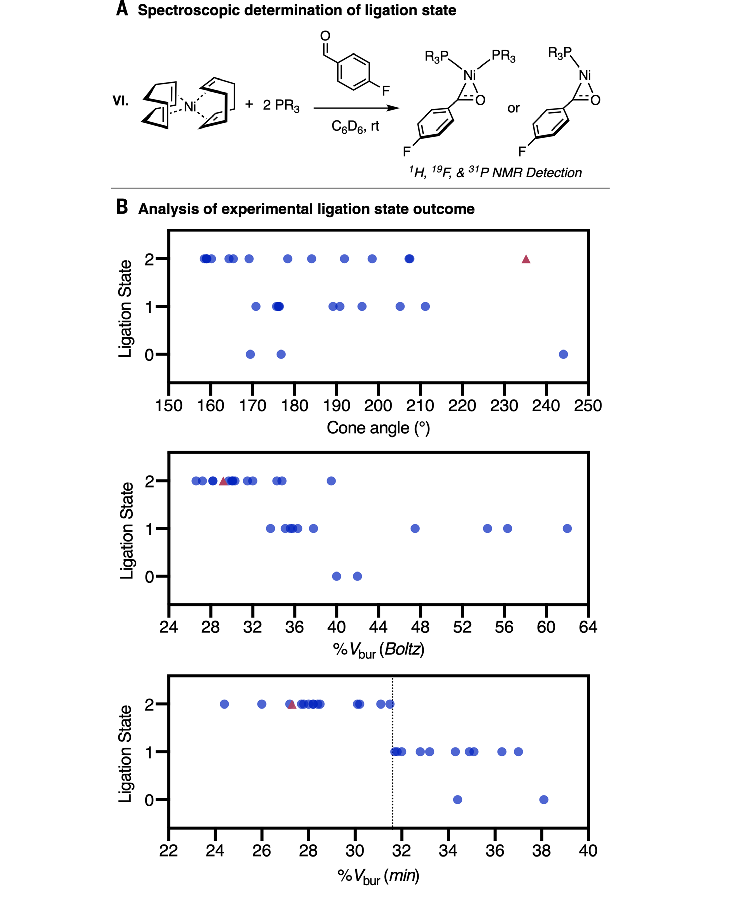
\includegraphics[width=\textwidth,height=0.68\textheight,keepaspectratio]{figures/chapter06-interrogate/02-newman-stonebraker-ligation-evidence-fig3.pdf}
  \caption{Independent ligation-state experiments plotted against the same steric descriptors used for the reactivity classification. Reproduced from Newman--Stonebraker \textit{et al.}, \textit{Science} (2021), Fig.~3.}
  \label{fig6-newman-ligation}
\end{figure}

\solution{4.2cm}{%
  \textbf{Locate the independent evidence.}
  \begin{itemize}
    \item On Fig.~\ref{fig6-newman-ligation}, separate the reaction outcome used to discover the boundary from the spectroscopic observation used to test the hypothesis.
    \item Draw the same approximate threshold used in Fig.~\ref{fig6-newman-cliff}.
    \item Mark a ligand whose behaviour would falsify a simple one-boundary interpretation.
  \end{itemize}
}\begin{figure}[htbp]
  \centering
  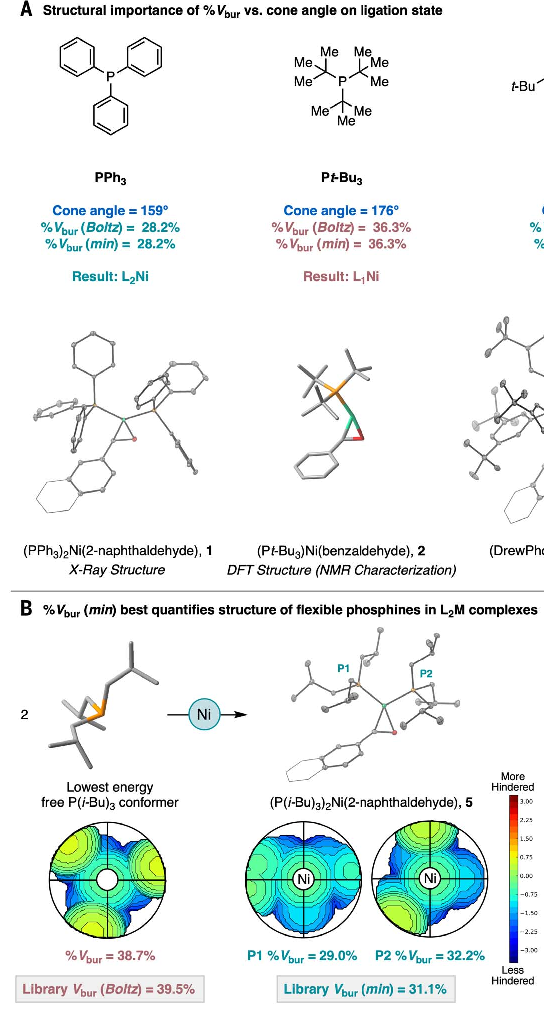
\includegraphics[width=\textwidth,height=0.70\textheight,keepaspectratio]{figures/chapter06-interrogate/03-newman-stonebraker-mechanistic-tests-fig4.pdf}
  \caption{Structural and computational tests of the proposed buried-volume/ligation-state relationship. These panels extend the argument beyond a statistical boundary. Reproduced from Newman--Stonebraker \textit{et al.}, \textit{Science} (2021), Fig.~4.}
  \label{fig6-newman-tests}
\end{figure}

\solution{4.6cm}{%
  \textbf{Label each kind of evidence in Fig.~\ref{fig6-newman-tests}.}
  \begin{itemize}
    \item Write ``structure'', ``spectroscopy'', ``calculation'', or ``reactivity'' beside each relevant panel.
    \item Draw arrows only where one observation genuinely supports the next inference.
    \item Put a question mark beside any step that still depends on interpretation rather than direct observation.
  \end{itemize}
}

The order of reasoning is crucial:

\solution{3.4cm}{%
  \centering
  reaction data $\longrightarrow$ statistical boundary $\longrightarrow$ chemical hypothesis\\[0.7em]
  $\longrightarrow$ independent organometallic/spectroscopic test\\[0.7em]
  $\longrightarrow$ mechanistic evidence
}

If the independent experiment had contradicted the proposed ligation-state change, the threshold could still have retained predictive value.
Its mechanistic interpretation would have failed.
Prediction and explanation can therefore separate without either becoming worthless.

\begin{conceptbox}
  \keypoint{Feature importance is not mechanistic evidence.}
  A descriptor can identify a reproducible chemical boundary.
  Mechanistic interpretation requires an intervention or independent measurement that tests the proposed chemical cause.
\end{conceptbox}

The use of $\%V_{\mathrm{bur}}(\min)$ also reminds us that representation is part of the chemical hypothesis.
The minimum across an ensemble asks whether the ligand can access a compact conformation that permits a particular ligation state.
A Boltzmann average asks a different question about the typical population.
The aggregation rule is not merely data processing; it expresses a proposed connection between conformational behaviour and reactivity.

% Suggested timing: 39--50 min
\section{Case study: when apparently good models do not transfer}

Kalikadien, Valsecchi, and co-workers generated up to 3552 measurements for rhodium-catalysed asymmetric hydrogenation using a standard library of 192 chiral rhodium precatalysts and five model substrates under varying conditions.\mcite{Kalikadien2024}
A curated subset of 960 observations was used for predictive modelling.
The high-throughput dataset contained many more low-conversion and low-selectivity outcomes than the corresponding literature record.
That difference is itself important: publication and selection practices change the response distribution presented to a model.

\begin{figure}[htbp]
  \centering
  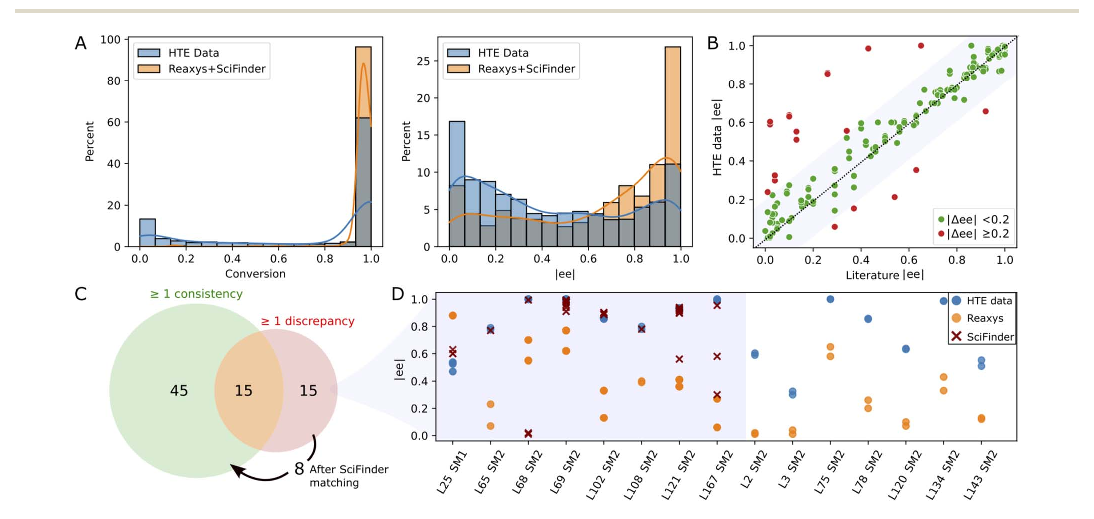
\includegraphics[width=\textwidth,height=0.66\textheight,keepaspectratio]{figures/chapter06-interrogate/04-kalikadien-hte-vs-literature-fig3.pdf}
  \caption{Comparison of the high-throughput and literature response distributions, including matched-condition consistency. The literature record and systematic screen present different chemical populations to a model. Reproduced from Kalikadien, Valsecchi \textit{et al.}, \textit{Chemical Science} (2024), Fig.~3.}
  \label{fig6-kalikadien-distribution}
\end{figure}

\solution{4.0cm}{%
  \textbf{Annotate selection bias directly on the distributions.}
  \begin{itemize}
    \item Shade the low-conversion and low-selectivity outcomes that a success-focused literature set underrepresents.
    \item Circle matched conditions where the records disagree.
    \item Write one consequence for classification and one for regression.
  \end{itemize}
}

Conversion was strongly near-binary, whereas enantioselectivity, represented as $\Delta\Delta G^{\ddagger}$, was treated as a continuous response.
The study compared less expensive molecular representations with automated quantum-chemistry-derived catalyst descriptors.
It also separated two validation questions.

\subsection{In-domain prediction}

In-domain tests placed examples from the same overall mixture of catalyst and substrate families in training and test sets.
For conversion, some useful predictive performance was possible.
Simple representations could perform as well as more expensive descriptors.
That result does not show that quantum descriptors are generally unhelpful.
It shows that additional calculation did not automatically add information relevant to this particular in-domain task.

\subsection{Out-of-domain prediction}

The stronger test withheld target substrates so that the model had to transfer from other substrates.
Performance was limited across representations.
Even expensive descriptors did not rescue prediction for genuinely new substrate chemistry.
The models could differentiate ligands represented in the data, but did not learn a transferable description of how catalyst, substrate, and conditions jointly controlled the new reaction.

\begin{figure}[htbp]
  \centering
  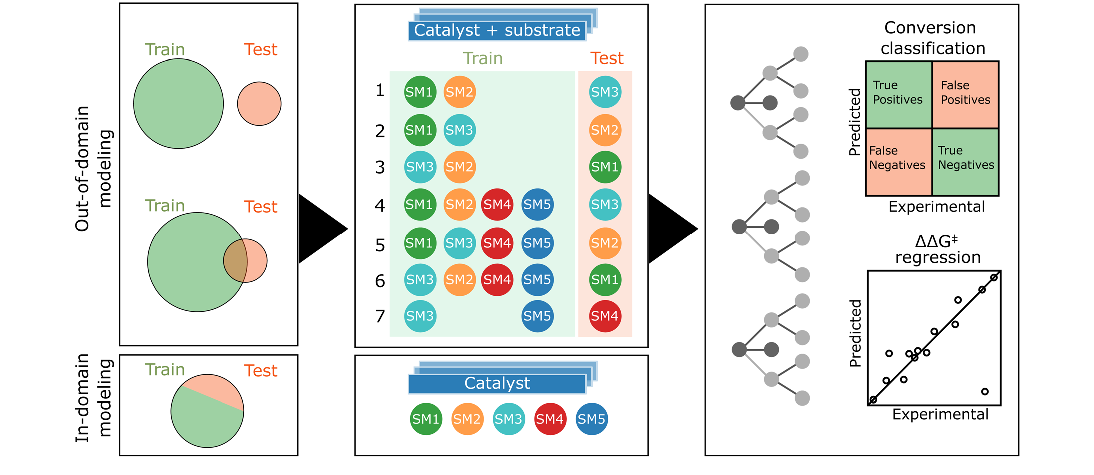
\includegraphics[width=\textwidth,height=0.50\textheight,keepaspectratio]{figures/chapter06-interrogate/05-kalikadien-in-vs-out-domain-fig6.pdf}
  \caption{Validation designs for in-domain, partially out-of-domain, and fully out-of-domain prediction. The chemical component held out determines the strength of the claim. Reproduced from Kalikadien, Valsecchi \textit{et al.}, \textit{Chemical Science} (2024), Fig.~6.}
  \label{fig6-kalikadien-splits}
\end{figure}

\solution{4.0cm}{%
  \textbf{Write the claim beside each validation design.}
  \begin{itemize}
    \item Mark which catalyst and substrate identities occur in both training and test data.
    \item Shade the completely withheld substrate family.
    \item Rank the panels from interpolation to strongest component transfer.
  \end{itemize}
}\begin{figure}[htbp]
  \centering
  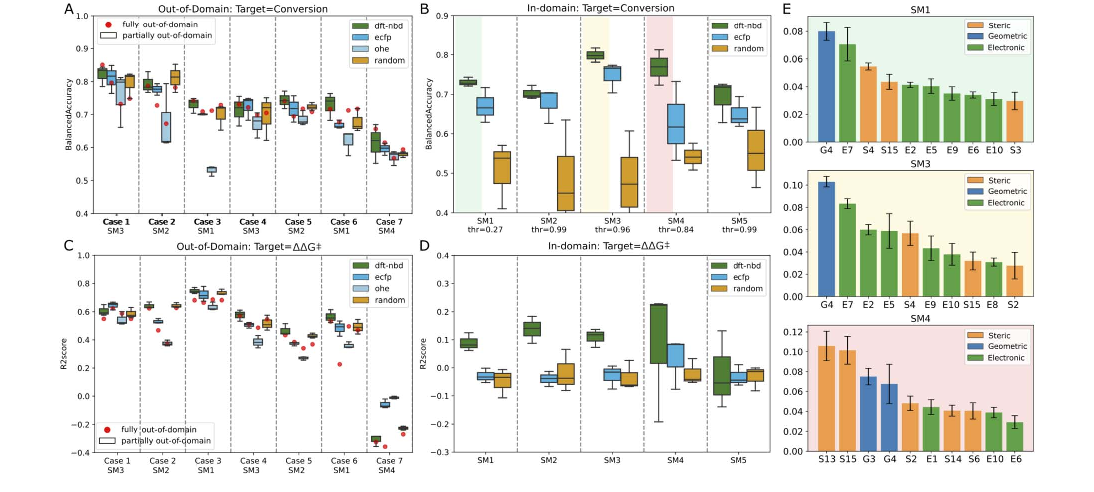
\includegraphics[width=\textwidth,height=0.52\textheight,keepaspectratio]{figures/chapter06-interrogate/06-kalikadien-model-performance-fig7.pdf}
  \caption{Model performance for in-domain and out-of-domain tasks, together with feature importance. Descriptor sophistication does not compensate automatically for missing chemical diversity. Reproduced from Kalikadien, Valsecchi \textit{et al.}, \textit{Chemical Science} (2024), Fig.~7.}
  \label{fig6-kalikadien-performance}
\end{figure}

% Reuse existing Figures 5.6--5.9: response distributions, in-domain/out-of-domain split,
% performance comparison, and HTE-versus-literature distribution.
\solution{5.0cm}{%
  \textbf{Connect the validation design to the observed performance.}
  \begin{itemize}
    \item on the in-domain panel, circle repeated catalyst and substrate families shared across training and test rows;
    \item on the out-of-domain panel, shade the withheld substrate family;
    \item write beside each panel the claim it can support;
    \item on the response histogram, mark the negative or poor outcomes absent from a success-biased literature set.
  \end{itemize}
}

\solution{3.8cm}{%
  \textbf{Interpret the failure.} Choose among the following and justify your choice:
  \begin{enumerate}
    \item the algorithm is insufficiently complicated;
    \item the catalyst descriptors are too cheap;
    \item the training data do not contain enough substrate diversity to learn the desired transfer;
    \item the representation omits catalyst--substrate interactions or mechanistic information.
  \end{enumerate}
  More than one can contribute, but model complexity alone does not solve missing chemical information.
}

This case corrects a common misunderstanding.
High apparent performance under random splitting does not demonstrate generalisation to new chemistry.
Nor does a descriptor become trustworthy merely because it is physically motivated or computationally expensive.
The validation design must reproduce the chemical novelty that the model will face.

% Suggested timing: 50--55 min
\section{Representation can change with the reacting complex}

Baidun and co-workers examined how model choice and conformational sampling affect descriptors for rhodium-catalysed acrylate hydrogenation.\mcite{Baidun2024}
They compared a generic precatalyst-like structure containing norbornadiene with a catalyst--substrate complex containing methyl 2-acetamidoacrylate across 11 rhodium catalysts with bidentate bisphosphine ligands.

\begin{figure}[htbp]
  \centering
  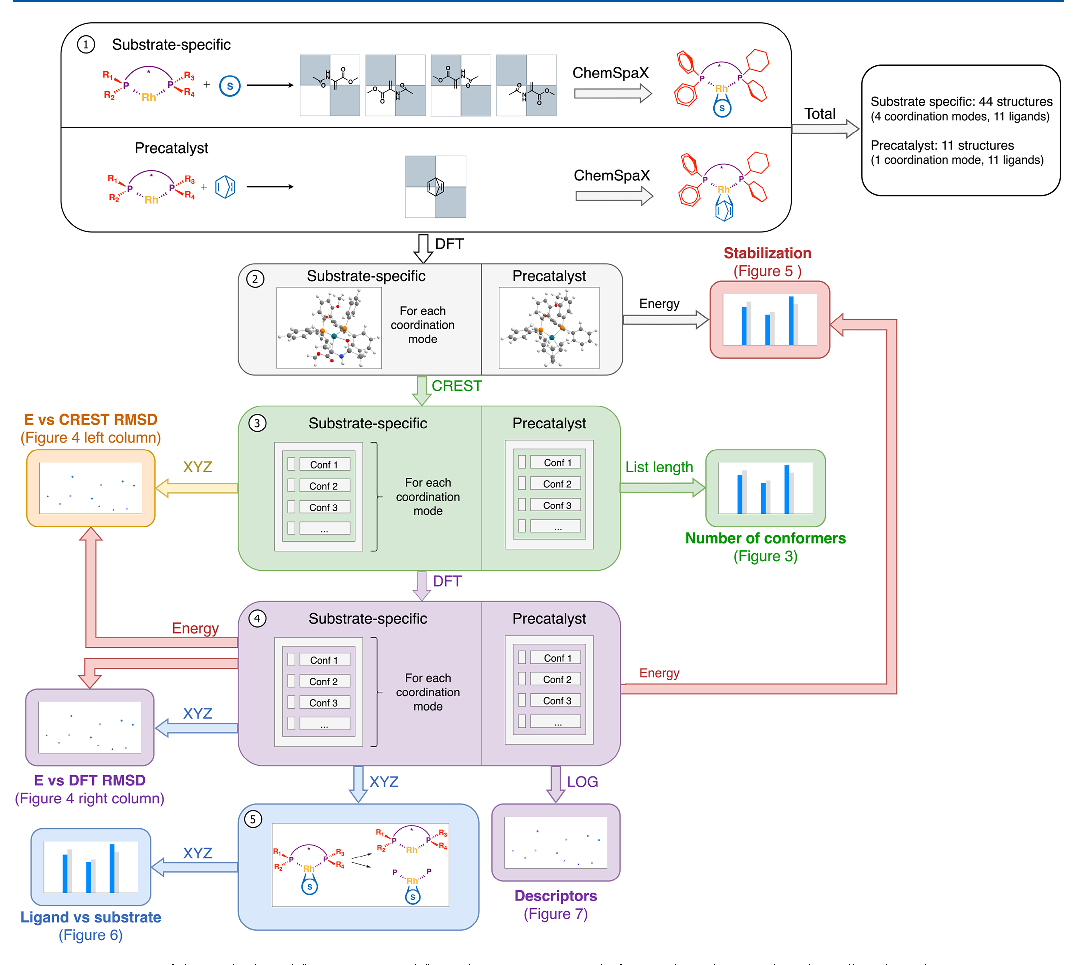
\includegraphics[width=\textwidth,height=0.70\textheight,keepaspectratio]{figures/chapter06-interrogate/07-baidun-conformer-workflow-fig2.pdf}
  \caption{Workflow for generating catalyst--substrate complexes, searching conformers, optimising structures, and calculating descriptors. The represented chemical object is a modelling decision. Reproduced from Baidun \textit{et al.}, \textit{J. Phys. Chem. C} (2024), Fig.~2.}
  \label{fig6-baidun-workflow}
\end{figure}

\solution{4.2cm}{%
  \textbf{Trace where representation choices enter the workflow.}
  \begin{itemize}
    \item Circle the first step at which substrate coordination is specified.
    \item Mark where conformers may be lost or retained.
    \item Write which chemical interactions a free-ligand representation would omit.
  \end{itemize}
}

The substrate-specific complex altered the number, energy, and geometry of accessible conformers.
Counterintuitively, binding a relatively rigid substrate could increase conformational diversity in the ligand framework.
Electronic and geometric descriptors therefore depended on which chemical complex was chosen for calculation and how its conformer ensemble was summarised.

\begin{figure}[htbp]
  \centering
  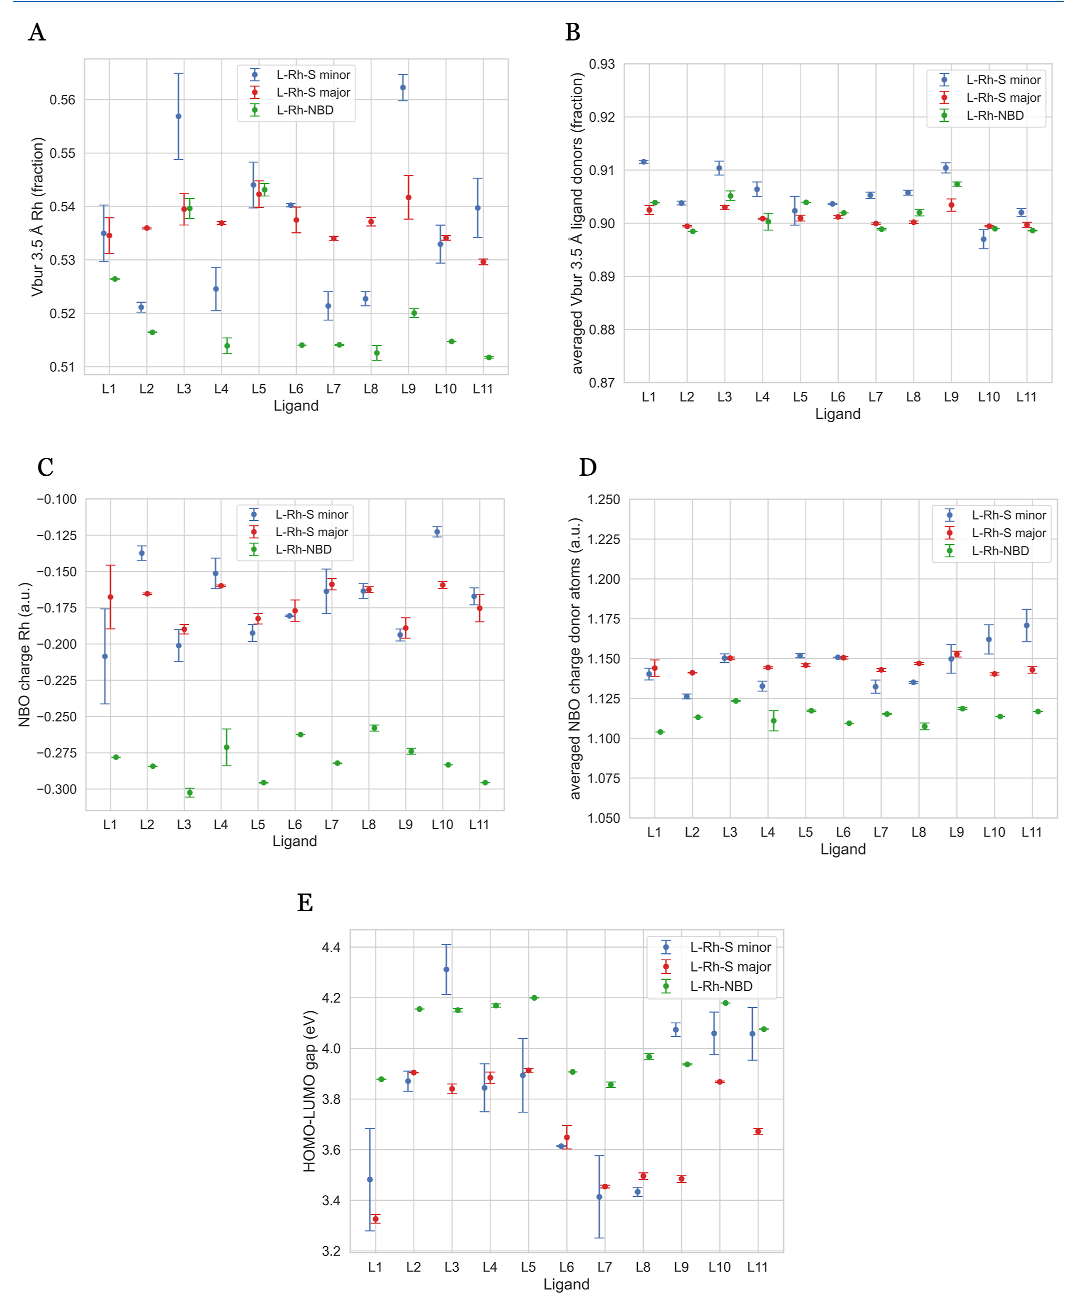
\includegraphics[width=\textwidth,height=0.72\textheight,keepaspectratio]{figures/chapter06-interrogate/08-baidun-descriptor-dependence-fig7.pdf}
  \caption{Selected descriptors calculated for substrate-bound complexes and a generic precatalyst ensemble. The descriptor value changes with represented state and conformational averaging. Reproduced from Baidun \textit{et al.}, \textit{J. Phys. Chem. C} (2024), Fig.~7.}
  \label{fig6-baidun-descriptors}
\end{figure}

\solution{4.0cm}{%
  \textbf{Compare like with like across Fig.~\ref{fig6-baidun-descriptors}.}
  \begin{itemize}
    \item Choose one descriptor and connect its values for the three represented states.
    \item Mark a ligand whose apparent position in descriptor space changes substantially.
    \item Finish: ``A narrow model confidence interval is misleading here if \ldots''
  \end{itemize}
}

\solution{3.8cm}{%
  \textbf{Draw the representation choice.}\\[0.4em]
  \begin{center}
    free ligand $\neq$ generic precatalyst $\neq$ substrate-bound catalytic complex
  \end{center}
  Under each structure, list which chemical interactions are present and which are omitted.
}

This does not mean that every model must use the most expensive substrate-specific quantum calculation.
It means that model uncertainty is only one source of uncertainty.
If the represented structure is chemically inappropriate, a narrow statistical confidence interval can create false precision.

\begin{warningbox}
  \keypoint{Uncertainty from the fitted model does not include every form of chemical ignorance.}
  Missing conformers, unrepresented catalyst states, mechanism changes, phase changes, and analytical failures can all lie outside the model's stated uncertainty.
\end{warningbox}

% Suggested timing: 55--60 min
\section{From model output to the next chemical experiment}

When a model disagrees with an experiment, there are several possible responses.
One is to increase model complexity.
Another is to inspect the experiment and representation.
A third is to design a new chemical test that distinguishes competing explanations.
The third response is often the most scientifically productive.

\solution{4.8cm}{%
  \textbf{Before trusting a chemical prediction, ask:}
  \begin{enumerate}
    \item What chemistry generated the training data?
    \item Where is the candidate in the representation actually used by the model?
    \item Is the response interpolated or extrapolated?
    \item Was this kind of component or scaffold novelty tested?
    \item Could speciation, mechanism, phase, or analytical behaviour change?
    \item Are residuals structured by chemical family or condition?
    \item Is the claim predictive or mechanistic?
    \item What independent experiment could falsify the proposed interpretation?
  \end{enumerate}
}

A model can therefore contribute to physical-organic chemistry in at least three ways.
It can predict an unmeasured response inside a tested domain.
It can expose a pattern, residual, or cliff that suggests missing chemistry.
It can rank experiments that would distinguish competing explanations.
Only the first of these is obtained from predictive accuracy alone.

\section{Summary}

Applicability domain is not an algorithm property; it is a claim about which chemistry has been sampled, represented, and tested.
Response-range, representation, component, scaffold, and mechanistic extrapolation are different risks.
Residuals and reactivity cliffs should be read using the identities of the reactions that generated them.
The Newman-Stonebraker study shows the productive sequence from statistical boundary to chemical hypothesis to independent spectroscopic and organometallic evidence.
The Kalikadien study shows that strong in-domain performance and expensive descriptors do not guarantee transfer to a withheld substrate family.
The Baidun study shows that descriptors depend on the chemical structure and conformer ensemble chosen for representation.
A model becomes chemically informative when it motivates experiments capable of confirming or falsifying the proposed interpretation.
